\documentclass[a4paper, 12pt]{article}
\usepackage{titling}
\usepackage{array}
\usepackage{booktabs}
\usepackage{enumitem}
\usepackage{graphicx}
\usepackage{hyperref}
\usepackage{amssymb}
\usepackage{listings}
\setlength{\heavyrulewidth}{1.5pt}
\setlength{\abovetopsep}{4pt}
\setlength{\parindent}{0pt}
\graphicspath{{.}}

\usepackage[margin=1in]{geometry}

% Must be after geometry
\usepackage{fancyhdr}
\pagestyle{fancy}
\fancyhf{}
\rhead{SEE Assignment 1}
\lhead{P.Lukin, E. Ovchinnikova}
\cfoot{\thepage}

\setlength{\droptitle}{-5em}

\title{Scientific Experimentation and Evaluation  \\
				Assignment: 1.1}
\author{Petr Lukin, Evgeniya Ovchinnikova}
\date{Lecture date: $04^{th}$ October 2016}

\begin{document}



\maketitle

\section{Construct the “simple robot” shown on the instruction sheet included in the LEGO construction
kit.}

We have assembled the robot in accordance to the instruction that is shown in Fig \ref{fig:robot}:
\begin{figure}[h]
  \centering
  \caption{Assembled Lego NXT robot with two light sensors. Front and side views.\label{fig:robot}}
  \includegraphics[width=0.8\textwidth]{LegoNXT}
\end{figure}

\section{Equip your robot with a pen, such that you can mark the position of the robot at its stop
position.}
As it is shown in Fig.\ref{fig:robot}, the robot is equipped with two light sensors that substitute laser pointers. NXT light sensors emit bright red light. We have narrowed the light spot and obtained 2 small accurate red dots that mark the position of the robot with a sufficient precision. After the robot stops, pen or pencil is used to mark position by hand. The advantage of this method is that the robot won't be moved in the moment of position measurement, as it can easily be moved when a pen touches the surface. Additionally, the robot has smaller construction: lights don't vibrate as long 'hand' with two pencils. 

\section{Verify your robot is running LeJOS and program it to run for a certain
distance.}
We have installed and tested LeJOS. The test was performed with the following program for forward motion:

\begin{lstlisting}

package LegoNXT;

import lejos.nxt.LightSensor;
import lejos.nxt.Motor;
import lejos.nxt.SensorPort;
import lejos.robotics.navigation.DifferentialPilot;
import lejos.robotics.navigation.MoveController;
import lejos.util.Delay;

public class goStraight {

        public static void main(String[] args) {
                double arcRad = 30;
                double angle = 90;
                LightSensor lightSens1 = new LightSensor(SensorPort.S1);
                LightSensor lightSens2 = new LightSensor(SensorPort.S2);
                DifferentialPilot dp = new DifferentialPilot
                (MoveController.WHEEL_SIZE_NXT1, 18, Motor.B, Motor.C,
                true);
                lightSens1.setHigh(100);
                lightSens2.setHigh(100);
                Delay.msDelay(5000);
                dp.setTravelSpeed(10);
                dp.travel(-Math.PI*2*arcRad*angle/360);
                dp.stop();
                Delay.msDelay(10000);
        }
}

\end{lstlisting}
\section{What and how we are planning to do.}
We are planning to observe the motion model of Lego NXT robot with a differential drive. Based on these observations we will obtain a distribution of final poses and calculate motion parameters.\\
The measuring system is following: the differential drive robot with two light sensors with narrow window for light emitting so it would emit only a point of light and a large sheet of paper with a coordinate system and two "garage" points which are determining the initial position of the robot - the light points must be on these points. On the paper sheet we can mark the robot's position using a pen that is not attached to the robot. To measure the coordinates of the robot's positions we are going to use a ruler and to store these results we are going to use a table in a LibreOffice Calc file.\\
The measuring method is the following: we are planning to estimate the position of the robot based on positions of two points of light emitted by light sensors. The starting position, the "garage", will also be marked as two points on the paper. 
Base coordinate frame is located as shown in Fig.\ref{fig:frame}:

\begin{figure}[h]
  \centering
  \caption{Base coordinate frame.\label{fig:frame}}
  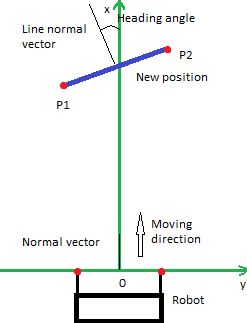
\includegraphics[width=0.4\textwidth]{frame}
\end{figure}

Initial position $X_0 = (0,0)$, heading angle $\phi = 0$. After measuring final coordinates of 2 red dots $P_1 = (x_1,y_1)$ and $P_2=(x_2,y_2)$, the robot's coordinates will be calculated:

\begin{equation}
X = (\frac{x_1+x_2}{2},\frac{y_1+y_2}{2}).
\end{equation}

Heading angle of the robot will be calculated as angle between normal vector $(1,0)$ and normal vector to line that goes through points $P_1,P_2.$

\begin{equation}
\phi = \arccos(\frac{y_2-y_1}{\sqrt{(y_2-y_1)^2+(x_1-x_2)^2}}).
\end{equation}


The measurement result will be obtained by conducting three series of experiments (around 30 times each): forward motion, left arc motion, right arc motion. After each of those experiments we measure the coordinates of the light points (measured value).  For the forward motion the program above will be used for the left and right motions the following programs will be used:

\begin{lstlisting}
package LegoNXT;

import lejos.nxt.Motor;
import lejos.nxt.SensorPort;
import lejos.robotics.navigation.DifferentialPilot;
import lejos.robotics.navigation.MoveController;
import lejos.util.Delay;
import lejos.nxt.LightSensor;

public class goLeft {

        public static void main(String[] args) {
                double arcRad = 30;
                double angle = 90;
                LightSensor lightSens1 = new LightSensor(SensorPort.S1);
                LightSensor lightSens2 = new LightSensor(SensorPort.S2);
                DifferentialPilot dp = new DifferentialPilot
                (MoveController.WHEEL_SIZE_NXT1, 18, Motor.B,
                Motor.C, true);
                lightSens1.setHigh(100);
                lightSens2.setHigh(100);
                Delay.msDelay(5000);
                dp.setTravelSpeed(10);
                dp.arc(-arcRad, angle);
                dp.stop();
                Delay.msDelay(10000);
        }
}

***

package LegoNXT;

import lejos.nxt.LightSensor;
import lejos.nxt.Motor;
import lejos.nxt.SensorPort;
import lejos.robotics.navigation.DifferentialPilot;
import lejos.robotics.navigation.MoveController;
import lejos.util.Delay;

public class goRight {

        public static void main(String[] args) {
                double arcRad = 30;
                double angle = 90;
                LightSensor lightSens1 = new LightSensor(SensorPort.S1);
                LightSensor lightSens2 = new LightSensor(SensorPort.S2);
                DifferentialPilot dp = new DifferentialPilot
                (MoveController.WHEEL_SIZE_NXT1, 18, Motor.B,
                 Motor.C, true);
                lightSens1.setHigh(100);
                lightSens2.setHigh(100);
                Delay.msDelay(5000);		
                dp.setTravelSpeed(10);
                dp.arc(arcRad, -angle);
                dp.stop();
                Delay.msDelay(10000);
        }
}

\end{lstlisting}
\section{Which difficulties we expect.}
\begin{itemize}
\item First difficulty that we expect is slightly different wheel diameter and uneven work of the motors. NXT Lego robots usually have problems because of slightly unsynchronized motor work. In this case the forward motion will be not exactly straight and arcs will have slightly wrong parameters.
\item Another possible difficulty in the measurement can be caused by incline of the surface, on which we put the sheet of paper, or the paper itself. In this case we could have the same problems as in previous case.
\item Since robot is shaking while moving, light sensors can slightly change their positions. In this case on or the both points can be moved and we estimate the position of the robot incorrectly.
\item Imperfection of the coordinate grid and a ruler that will cause a systematic error that we must take into account.
\item Imperfection of a light point and a pen - both, the point, and a pen are not material points, so they have a certain diameter that will add a systematic error.
\item Measuring facility that consists of lights, eyes, pens has too many objects that add extra noise to measurand.
\end{itemize}



\end{document}
